\documentclass[twoside,a4paper,12pt]{article}


\usepackage[utf8]{inputenc}
\usepackage[english]{babel} 
\usepackage{polski}
\usepackage{helvet}
\usepackage{graphicx}
\usepackage{color}
\usepackage{geometry}
\usepackage{url}
\usepackage[hidelinks]{hyperref}
\usepackage{minted}
\usepackage{amsmath}
\usepackage{amsfonts}
\usepackage{csquotes}
\usepackage{microtype}
\usepackage{prettyref}
\usepackage{overpic}
\usepackage{svg}

\newrefformat{fig}{Figure~[\ref{#1}]}
\usepackage{subcaption}

\geometry{hmargin={2.5cm, 2cm}, height=10.0in}
\usepackage{epstopdf}

\usepackage{multicol}
\usepackage[toc,page]{appendix}
\usepackage{caption}

\usepackage{emptypage}
\pretocmd{\section}{\cleardoublepage}{}{}

\newcommand{\setSupervisor}[1]{
    \newcommand{\supervisor}{#1}
}
\newcommand{\setFaculty}[1]{
    \newcommand{\faculty}{#1}
}

\newcommand{\setDepartment}[1]{
    \newcommand{\department}{#1}
}

\newcommand{\setReviewer}[1]{
    \newcommand{\reviewer}{#1}
}

\makeatletter
\renewcommand{\maketitle}{\begin{titlepage}
        \includegraphics[height=37.5mm]{img/agh_nzw_a_pl_1w_wbr_cmyk}\\
        \rule{30mm}{0pt}
        {\large \textsf{\department}}\\
        \rule{\textwidth}{3pt}\\
        \rule[2ex]
        {\textwidth}{1pt}\\
        \vspace{7ex}
        \begin{center}
            {\LARGE \bf \textsf{Engineering thesis}}\\
            \vspace{13ex}
            % --------------------------- IMIE I~NAZWISKO -------------------------------
            {\bf \Large \textsf{\@author}}\\
            \vspace{3ex}
            {\sf\small field of study:} {\bf\small \textsf{\faculty}}\\
            \vspace{1.5ex}
            \vspace{10ex}
            %% ------------------------ TYTUL PRACY --------------------------------------
            {\bf \huge \textsf{\@title}}\\
            \vspace{14ex}
            %% ------------------------ OPIEKUN PRACY ------------------------------------
            {\Large Thesis supervisor: \bf \textsf{\supervisor}}\\
            \vspace{22ex}
            {\large \bf \textsf{Kraków, \@date}}
        \end{center}
    \end{titlepage}%
}
\makeatother

\setminted[c]{frame=lines,
    framesep=2mm,
    baselinestretch=1.2,
    fontsize=\footnotesize,
    linenos}


\author{Eryk Zarębski}
\title{An algorithm for classifying chemical elements using data collected with the X-ray fluorescence technique}
\setDepartment{Faculty of Physics and Applied Computer Science}
\setFaculty{Applied Computer Science}
\setSupervisor{prof. dr hab. inż. Tomasz Szumlak}
\setReviewer{dr inż. TODO}

\begin{document}
\pagestyle{empty}
\maketitle

\null
\newpage
\begin{abstract}
During recent years, deep learning models have proven their usability in numerous tasks that cannot be easily modeled using linear methods. The range of application areas begins with school projects, such as creating a binary classification model to differentiate between photos of cats and dogs, and extends to advanced applications like autonomous vehicles and Artificial General Intelligence (AGI)-like Large Language Models (LLM). In the field of material sciences, a novel method for non-invasive X-ray fluorescence (XRF) data acquisition has been developed. Although algorithms with proven efficacy for analyzing these spectra already exist, and unlike deep learning models, they are easily explainable, they also have shortcomings. For instance, the commonly used Region of Interest (ROI) technique encounters difficulties in detecting elements invisible in accumulated spectra, differentiating signals with very similar characteristic energies and obtaining information about their actual distribution in the signal. This paper presents an attempt to create a convolution neural network (CNN) based model for classifying chemical elements present in spectra acquired using X-ray fluorescence techniques. 
\end{abstract}

\pagestyle{plain}
\linespread{1.3}
\selectfont

\null
\newpage
\pagenumbering{roman}
\tableofcontents
\null
\newpage
% \mbox{}
\null
\newpage

\pagenumbering{arabic}

\section{Introduction}
% \subsection{X-ray fluorescence data acquisition method}
\subsection{Motivation}
The work presented in this paper builds upon contributions made by dr. inż. Bartłomiej Łach in his doctoral thesis entitled \emph{Rozwój systemu detekcyjnego do obrazowania przestrzennego rozkładu pierwiastków metodą fluorescencji rentgenowskiej}\cite{Lach2022}  (eng. \emph{Development of a detection system for spatial imaging of element distribution using X-ray fluorescence}).

His dissertation was dedicated to development of system for non-invasive analysis of works of art that uses X-ray radiation to carry out measurements. 
The system presented in paper was designed to provide a map of element distribution in the top layers of the object, offering essential information for analyzing the pigments used in the artwork. 
The result would be important knowledge for conservators of monuments and art, informing them about the object's state of preservation, quality of past maintenance processes, the assessment of the work's authenticity, and the expansion of previous state of knowledge.

Most popular technique to achieve such results, namely MA-XRF (\textbf{MA}cro \textbf{X-R}ay \textbf{F}luorescence), operate by scanning selected parts of art point by point. 
This method is characterized by high spatial and energetic resolution. 
However, due to usage of polycapillary lenses it is limited to performing scans on 2D surfaces. 
Another drawback is long measurement time. 
For example, scanning a painting with an area of $65 \times 45$ $\text{cm}^{2}$, a resolution of $1300 \times 900$ pixels, and a  dwell time of $10$ ms per pixel could take about $3.5$ hours.\cite{Alfeld2013}. 

An alternative method involves scanning not just a single point but multiple points within a specific area of the surface, utilizing FF-XRF (\textbf{F}ull-\textbf{F}ield \textbf{X-R}ay \textbf{F}luorescence). 
This approach was implemented in the DETART (\textbf{DET}ector for \textbf{ART}) data acquisition system. 
DETART not only can scan large portion of the surface (over $10e5$ pixels at the same time), but it is also capable of performing scans of 3D objects without losing spatial resolution thanks to near infinite depth of field provided by pinhole camera. 

After data acquisition part, the analysis can be performed. 
Łach proposed three different methods for analyzing data: "standard" ROI (\textbf{R}egion \textbf{O}f \textbf{I}nterest) method and two different machine learning algorithms: PCA (\textbf{P}rincipal \textbf{C}omponents \textbf{A}nalysis) and NFM (\textbf{N}on-negative \textbf{M}atrix \textbf{F}actorization). 
In this paper, a method based on deep learning instead will be proposed and tested. 

\subsection{Concept}
Concept of this thesis is heavily inspired by the work presented in \cite{Jones2022}. 
The authors of this article introduced the idea of a CNN (\textbf{C}onvolutional \textbf{N}eural \textbf{N}etwork) model tasked with classifying every sample measured with XRF as one pigment class. 
The model was initially trained on synthetic data generated by software, achieving an accuracy of 55\% when tested on real XRF spectra, and then 96\% after applying transfer learning using small quantity of real XRF samples.  
This approach has several advantages, such as full automation of the process, and high accuracy after applying transfer learning.
However, there are some downsides to consider:
\begin{itemize}
    \item The model can only classify pigments it has learned about
    \item It does not provide any information about signals coming from elements, which may offer some valuable insights about the studied object
\end{itemize}
A potential solution to these problems may be to shift the focus from classifying pigments to classifying elements. A multi-label classification approach might be used to assess existence of each learned element independently from the tested pigment. This approach is more similar to algorithms used in Łach's thesis.

\section{Methodology}
\subsection{Used Technologies}

All code developed during the project was written in the \texttt{python3} programming language. Google Colab was utilized as runtime environment, as it provides resources that allows rapid testing of DNN (Deep Neural Network) implementations. 
Google Colab also enabled easy sharing of interactive notebooks with the thesis supervisor.

The primary technologies and libraries used in the project include:
\begin{itemize}
    \item \texttt{python3} programming language.
    \item \texttt{pytorch} - Chosen as the deep learning framework due to the author's familiarity with it and its widespread adoption among researchers (over 60\% of new paper implementations use \texttt{pytorch} \cite{papersWithCodeTrends}).
    \item \texttt{hdbscan} - Implementation of the HDBSCAN (Hierarchical Density-Based Spatial Clustering of Applications with Noise) algorithm for data clusterization.
    \item \texttt{umap-learn} - Implementation of the UMAP (Uniform Manifold Approximation and Projection) algorithm for dimensionality reduction.
    \item \texttt{minisom} - Implementation of a SOM (Self-Organizing Map) algorithm for data clusterization.
    \item \texttt{scikit-learn}, \texttt{scipy}, \texttt{matplotlib}, \texttt{pandas}, \texttt{numpy} - Common tools used for data analysis in the \texttt{python} ecosystem.
\end{itemize}
\subsection{Key Algorithms}
\subsubsection{DNN Selection}

The initial choice for classifying XRF spectra involved utilizing a neural network from the ResNet family, specifically ResNet50. The selection of ResNet was arbitrary but justified by its reputation as a robust CNN architecture. Notably, ResNet architecture won the ImageNet Large Scale Visual Recognition Challenge in 2015 \cite{ImageNet2015}.

ResNet architecture is characterized by its ability to support very deep networks. This is attributed to the presence of residual connections, which allow each block of network for the learning of residual mappings $g(x) = f(x) - x$ rather than the usual mapping $f(x)$ \cite{d2lResnet}. 

If the desired mapping is identity mapping $f(x) = x$, then block must only learn mapping $g(x) = 0$, which is easy to learn. 
As a result it is hard to degrade performance of this architecture with increasing depth - see \prettyref{fig:residual-block}.

\begin{figure}[h] 
  \centering     
  \includesvg[width=0.8\textwidth]{img/residual-block.svg} 
  \caption{ The residual block (right) needs to learn the residual mapping $g(x) = f(x) - x$ , wheres regular block (left) must learn direct mapping $f(x)$. Source: \cite{d2lResnet}}
  \label{fig:residual-block}
\end{figure}

However, the original architecture of ResNet incorporates a \emph{global average pooling} operation just before the final fully connected layer. 
This operation calculates the average value over the spatial dimensions of a single feature map. 
In the case of adapting ResNet to work with 1D spectra, the input for global average pooling has a shape of (batch\_size, channels, features) and the output has shape (batch\_size, channels, 1). 
It means that due to averaging over features the spatial information is lost!

This resulted in the network not performing as expected, since peak positions in XRF spectra are crucial to identify elements. 
Furthermore, replacing global average pooling with a flattening operation was not feasible, as it would lead to \\ $\text{{channels}} \times \text{{features}} \times \text{{fully\_connected\_size}}$ total connections with the fully connected layer. 
For example, with an input vector of shape $(\text{{batch\_size}}, 2048, 128)$ (which was observed during development), this would result in approximately $5 \times 10^{8}$ trainable parameters, while default implementation of ResNet50 have only $\sim2.6 \times 10^7$ as a whole!

To address this problem, several possibilities were considered:
\begin{enumerate}
    \item Modifying the architecture of ResNet to further reduce dimensionality further using convolution and pooling operations.
    \item Reducing size of fully connected layer.
    \item Opting for a completely different architecture.
\end{enumerate}

While the two first options vere feasible, the decision was made to change used architecture completely. 
As a result, the author chose to use the ViT (Vision Transformer).

\subsubsection{Multi-Head Attention}
To understand ViT one ought to first understand how transformers work in general.
Transformer architecture was originally meant to be replacement for RNNs (Recurrent Neural Networks) \cite{Vaswani2017}.
Although transformers needs more training data (due to small inductive bias\footnote{e.g. ``In computer vision related tasks, the great success of convolutional neural networks (CNN) is often attributed to its inductive biases, such as locality and translation equivariance. \cite{Mormille2023}''. 
In contrast, transformers exhibit less inductive biases, enabling them to explore a broader hypothesis space. 
Consequently, they may converge to local optima and generalize poorly on unseen data, when trained on insufficient data.}) 
than recurrent networks to achieve similar results, they have significant advantage in terms of parallelization.

Unlike classic RNNs, which require the use of the hidden state calculated at time step $t-1$ to compute the hidden state at time step $t$, which makes them non-parallelizable, transformers are highly parallelized, thanks to \emph{multi-head attention}, which makes heavy use of matrix multiplication.

Multi-Head Attention works based on \emph{attention mechanism}, which is somewhat similar to a database query \cite{d2lAttentionMechanism}.
To explain it let's define a key-value database consisting of $(\mathbf{k}, \textbf{v})$ vector pairs which can be queried using $\mathbf{q}$ vector query: \[ D\overset{\text{def}}{=}\{(\mathbf{k_i}, \mathbf{v_i}) \mid i = 1, 2, \ldots, n\}.\]
Then attention over $D$ can be denoted as:
\[ \text{Attention}(\mathbf{q}, D) = \sum_{i=1}^{n}\text{a}(\mathbf{q}, \mathbf{k_i})\mathbf{v_i},\]
where $\text{a}(\mathbf{q}, \mathbf{k_i}) \in \mathbb{R}$ are attention weights.

If exactly one of the weights $\text{a}(\mathbf{q},\mathbf{k_i}) = 1$, while all others are $0$, then attention works like normal database query and returns value of $\mathbf{v_i}$ for $\mathbf{k_i}$ that matches $\mathbf{q}$.
In case that there are multiple non-zero weights then some linear combination of vectors is retrieved. 
For deep learning applications the following properties are desirable: $\sum_i \text{a}(\mathbf{q}, \mathbf{k_i}) = 1$ and $\text{a}(\mathbf{q}, \mathbf{k_i}) \ge 0$. To guarantee this behaviour, the Softmax function can be applied:

\[ \alpha(\mathbf{q}, \mathbf{k_i}) = \text{Softmax}(\text{a}(\mathbf{q}, \mathbf{k_i})) = \frac{\text{exp}(\text{a}(\mathbf{q}, \mathbf{k_i}))}{\sum_j \text{exp}(\text{a}(\mathbf{q}, \mathbf{k_j}))}.\]

The last thing to be defined is the attention scoring function $\text{a}(\mathbf{q}, \mathbf{k_i})$.
It is highly unlikely to find any exact match between $\mathbf{q}$ and $\mathbf{k_i}$, so $\text{a}(\mathbf{q}, \mathbf{k_i})$ must be defined as some similarity function between vectors in feature space.

Let's take a look at Gaussian similarity kernel, which is a non-linear function of euclidean distance:
\[\text{K}(\mathbf{x}, \mathbf{x'}) = \text{exp}(-\frac{\norm{\mathbf{x} - \mathbf{x'}}}{2\sigma}).\]
It has nice property of being bound between zero and one, unlike euclidean distance which could be anything and lead to numerical instabilities.
However, it has disadvantage of being computationally costly.

Now lets consider the kernel with substituted $\mathbf{q}$ and $\mathbf{k_i}$, exponentiation skipped, and in expanded form:

\[\text{k}(\mathbf{q}, \mathbf{k_i}) = -\frac{1}{2}\norm{\mathbf{q} - \mathbf{k_i}}^2 = \mathbf{q}^\intercal \mathbf{k_i} - \frac{1}{2}\norm{\mathbf{k_i}}^2 - \frac{1}{2}\norm{\mathbf{q}}^2.\]
The last term is constant across all values of $\mathbf{k_i}$ and due to normalization its presence don't affect the result. 
Therefore, it can be safely omitted. 
Similarly, the second term may be disregarded because batch/layer normalization effectively bounds $\norm{\mathbf{k_i}}$, ensuring a negligibly small impact on the final result \cite{d2lAttentionScoring}.

If we assume that $q \in \mathbb{R}^{d}$ and $k_i \in \mathbb{R}^d$, and that their elements are drawn from distribution $\mathcal{N}(\mu=0, \sigma^2=1)$, then their dot product will have mean zero and variance $d$.
After normalization by factor $\frac{1}{\sqrt{d}}$, the first commonly used attention function - \emph{scaled dot product attention} \cite{Vaswani2017} can be written down as:

\[\text{a}(\mathbf{q}, {\mathbf{k_i}}) = \frac{\mathbf{q}^\intercal \mathbf{k_i}}{\sqrt{d}}.\]
Final attention weights can be calculated by applying Softmax: 

\[\alpha(\mathbf{q}, \mathbf{k_i}) = \text{Softmax}(\text{a}(\mathbf{q}, \mathbf{k_i})) =\frac{\text{exp}(\frac{q^\intercal k_i}{\sqrt{d}})}{\sum_j \text{exp}(\frac{q^\intercal k_j}{\sqrt{d}})}.\]

To take advantage of parallelization, vector multiplication can be replaced with matrix multiplication. When computing attention for $n$ queries and $m$ key-value pairs, where both queries and keys have a length of $d_k$ (although it must not necessarily be the case), and values have a length of $d_v$, the following matrices must be defined: $Q \in \mathbb{R}^{n \times d_k}$, $K \in \mathbb{R}^{m \times d_k}$, and $V \in \mathbb{R}^{m \times d_v}$. These matrices will form a formula analogous to that of vectors:

\[\text{Attention}(Q, K, V) = \text{Softmax}(\frac{Q K^\intercal}{\sqrt{d}})V.\]

In practice, it was found that it is advantageous to combine multiple attention pooling outputs computed in parallel. 
In theory it may lead to capturing different behaviours of attention mechanism, e.g. capturing short-range and long-range dependencies within a sequence \cite{d2lMultiHeadAttention}.


A single output of attention pooling was originally referred to by the authors as a \emph{head}. 
multi-head attention can be calculated in following way: 
\[\text{MultiHeadAttention}(Q, K, V)  = \text{Concat}(head_1, head_2, \dots, head_n)W^O,\]
where $head_i = \text{Attention}(QW_i^Q, KW_i^K, VW_i^V) \in \mathbb{R}^{p_v}$, where $W_i^Q \in \mathbb{R}^{d_k \times p_k}$, $W_i^K \in \mathbb{R}^{d_k \times p_k}$, $W_i^V \in \mathbb{R}^{d_v \times p_v}$ and $W_i^O \in \mathbb{R}^{(hp_v) \times p_o}$ are learnable parameters.
To better manage computational cost, the input sizes for each head are parameterized in following manner: $p_k = p_v = p_o / h$, where $h$ is number of heads and $p_o$ is size of output of last fully connected layer. Thanks to that, computational cost don't increase with higher number of heads.

\subsubsection{ViT Architecture}
Multi-Head Attention is the most important concept used in transformer architecture, it is no different when it comes to Vision Transformer \cite{vitPaper}.
DNN architecture used to classify XRF spectra is slightly modified version of ViT, which was adapted to work with 1D input.

Most parts of the architecture remain unchanged.
Transformer encoder is implemented (\prettyref{lst:transformer_encoder}) in exactly the same way as in original paper - \prettyref{fig:transformer-encoder}.
In contrast to the original transformer encoder architecture \cite{Vaswani2017}, layer normalization in ViT is applied before all MHA and MLP (Multi Layer Perceptron) in order to enhance training effectiveness.
Moreover, the commonly used non-linear activation function ReLU (Rectified Linear Unit) is replaced with its smoother counterpart, GELU (Gaussian-Error Linear Unit).

\begin{figure}[H] 
  \centering     
  \includegraphics[width=0.3\textwidth]{img/transformer-encoder.png} 
  \caption{Transformer Encoder architecture. Source: \cite{vitPaper}}
  \label{fig:transformer-encoder}
\end{figure}

\newenvironment{longlistingA}{\captionsetup{type=listing, width=0.8\textwidth}}{}
\begin{longlistingA}
    \pythoncode{listings/transformer_encoder.py}
    \caption{Transformer Encoder block implementation. The implementation details were based on \cite{d2lViT}}
    \label{lst:transformer_encoder}
\end{longlistingA}
\vspace{12pt}

Several modifications were introduced in the remaining part (\prettyref{lst:vit}) of the original implementation - \prettyref{fig:original-vit-architecture}, \prettyref{fig:modified-vit-architecture}.

\begin{figure}[ht] 
  \centering     
  \includegraphics[width=0.6\textwidth]{img/vit_changed.png} 
  \caption{Modified ViT architecture.}
  \label{fig:modified-vit-architecture}
\end{figure}

\begin{figure}[H] 
  \centering     
  \includegraphics[width=0.7\textwidth]{img/original_vit.png} 
  \caption{Original ViT architecture. Source: \cite{vitPaper}}
  \label{fig:original-vit-architecture}
\end{figure}


The \texttt{[class]} token has been removed.
\texttt{[class]} token was an idea introduced in model BERT (Bidirectional Encoder Representations from Transformers) \cite{bertOriginal} and it was used as an input to classifying MLP.
However, due to small embedding and input size it was possible to remove it and replace with fully connected layer.
Additionally, the authors discovered that the \texttt{[class]} token was not inherently superior to other methods; other methods required just a distinct learning rate \cite{vitPaper}.

Another adjustment was to replace patch embedding using \texttt{nn.Conv2d} (2D convolution operation) with \texttt{nn.Conv1d}, because the input is not a 2D image but a 1D spectrum. 

Last but not least, the softmax function was replaced with the sigmoid function to enable the classification of multiple labels simultaneously.

\newenvironment{longlistingC}{\captionsetup{type=listing, width=0.8\textwidth}}{}
\begin{longlistingC}
    \pythoncode{listings/vit.py}
    \caption{ViT implementation. The implementation details were based on \cite{d2lViT}}
    \label{lst:vit}
\end{longlistingC}
\vspace{12pt}

\subsubsection{Self-Organizing Map}
Being able to classify elements in the spectrum is only part of the success. 
Data gathered using FF-XRF has a mean of around 20,000 photon counts per one spatial coordinate - see \prettyref{fig:matka-boska-photon-count}. 
When distributed over $\sim$4000 possible energy levels, it provides a rather noisy spectrum that may not yield correct classification. 
It would also come with long total inference time. 

\begin{figure}[H] 
  \centering     
  \includesvg[width=0.7\textwidth]{img/matka_boska_photon_count.svg} 
  \caption{Photon count in data gathered from the painting ``Mother of God with the Child Eating an Apple''}
  \label{fig:matka-boska-photon-count}
\end{figure}

To address this issues, one of the following strategies may be involved:
\begin{enumerate}
  \item Calculating the average of spectra in some small region.
  \item Calculating the average of clustered spectra.
\end{enumerate}

The first option is easier because clustering high-dimensional data is a daunting task due to the \emph{curse of dimensionality}.

Available options are highly limited, but they do exist. 
One algorithm that can tackle high-dimensional clustering is the SOM (Self-Organizing Map) algorithm, which is an unsupervised machine learning algorithm based on a neural network. 
It is mainly used for visualization of feature-rich data because it reduces its dimensionality to (usually) 2D map, but has been proven to work well as clustering algorithm for XRF spectra \cite{Kogou2020}.

The algorithm works in the following way \cite{somTutorial}: 
\begin{enumerate}
    \item $n$ weights $\mathbf{w_i}$ of the same length as feature vectors are initialized.
    \item Weights are distributed over a 2D map using a specified topology, such as a square, hexagonal, or random grid.
    \item A vector $\mathbf{d}$ is chosen from the training data set.
    \item $\mathbf{d}$ is compared to each node $\mathbf{w_i}$ on the map using a distance function, such as the $l_2$ norm or $l_1$ norm. The node with the closest distance is designated as the BMU (Best Matching Unit).
    \item The neighborhood of the BMU is calculated.
    \item The BMU and all nodes in the neighborhood are updated, making them more similar to $\mathbf{d}$.
    \item The algorithm is repeated from step 3 for a specified number of iterations.
\end{enumerate}

The weights are updated using following equation \cite{somWikipedia}:
\[\mathbf{w}_i^{s+1} = \mathbf{w}_i^s + \theta(u, v, s) \cdot \alpha(s) \cdot (\mathbf{d} - \mathbf{w}_i^s).\]
Here, $s$ represents the number of iterations, $u$ the index of the BMU and $v$ the index of the node on the map (may be the same as $u$). 
The function $\theta(u, v, s)$ represents the neighborhood function and states that the BMU is updated the most and farther neighbors are updated less. 
An example of a neighborhood function could be a Gaussian kernel. 
The function $\alpha(s)$ represents the learning rate schedule.

Although algorithm is fairly simple, the most popular python packages don't have its implementation, and the most popular implementation - package \texttt{minisom} had too large RAM memory requirements, which lead to crashing Colab environment with 50GB of memory.
Because of that its basic implementation was written using python and \texttt{numpy} package - \prettyref{lst:som}. 

\newenvironment{longlistingB}{\captionsetup{type=listing, width=0.8\textwidth}}{}

\begin{longlistingB}
    \pythoncode{listings/som.py}
    \caption{Simple Self-Organizing Map implementation. Graphical representation of weights update step can be seen in \prettyref{fig:som}}
    \label{lst:som}
\end{longlistingB}
\vspace{12pt}

\begin{figure}[H] 
    \centering     
    \begin{overpic}[width=0.6\linewidth]{img/som.png}
        \put(56,39){\textcolor{black}{\fontsize{20}{16}\selectfont $\mathbf{d}$}}
    \end{overpic}
    \caption{Updating the best matching unit (BMU) and its neighbours towards the input sample $\mathbf{d}$. Source: \cite{somGraphic}}
    \label{fig:som}
\end{figure}

\subsubsection{UMAP and HDBSCAN Clustering Pipeline}
Unfortunately, clustering the data with SOM showed some weird artifacts in all analyzed samples.
It was the reason to find alternative clusterization method to ensure that the artifacts were not caused by the algorithm.
After some research it was found that UMAP (Uniform Manifold Approximation and Projection) $\rightarrow$ HDBSCAN (Hierarchical Density-Based Spatial Clustering of Applications with Noise) clustering pipeline should also work with large datasets of high dimensional data. 

According to the UMAP documentation it does not produce clean, spherical clusters, so algorithms like K-Means dont't work well on its output. 
UMAP comes with uniform density assumption, so density is not preserved correctly. 
However, UMAP contracts connected components of the manifold together, which should be easily picked out by algorithms like HDBSCAN.
It offers significant improvements over algorithms like t-SNE for clustering, as it preserves more global structure and creates meaningful separation between connected components, resulting in more meaningful clusters \cite{umapFaq}. 

The HDBSCAN algorithm is a follow-up to the DBSCAN algorithm. 
The key distinction between HDBSCAN and DBSCAN lies in HDBSCAN's ability to determine clusters with different densities.

Due to the complexity of these algorithms and the author's lack of familiarity with topology, further explanation of the algorithms will not be provided here. 
Interested readers can refer to their respective papers \cite{Campello2013}, \cite{McInnes2018}, or their documentation.
\subsection{Artificial Data Generation}
To train a DNN in a supervised fashion, one must be in possession of labeled data. 
Acquisition of such data is by and large beyond the scope of this thesis. 
The only feasible way to acquire large enough amounts of data is to generate it. 
Such efforts have already been made in \cite{Jones2022}, and a similar approach is used here.

To generate training data, a special function has been created - \prettyref{lst:data_generation}. 

\newenvironment{longlistingD}{\captionsetup{type=listing, width=0.8\textwidth}}{}
\begin{longlistingD}
    \pythoncode{listings/data_generation.py}
    \caption{Function for training data generation}
    \label{lst:data_generation}
\end{longlistingD}
\vspace{12pt}

The function creates artificial spectra by adding multiple gaussians in form: \[\mathcal{N}(\mu + \mathcal{U}(-e_\mu^{\text{global}}, e_\mu^{\text{global}}) + \mathcal{U}(-e_\mu^{\text{local}}, e_\mu^{\text{local}}), \sigma + \mathcal{U}(-e_\sigma^{\text{local}}, e_\sigma^{\text{local}})),\]
that represents a single peaks of element in spectrum, where $\mu$ is the energy of peak, $\sigma$ is the standard deviation and $e$ terms are respective error values. Additionally, the arbitrary exponential is added to the sum of gaussians to account for background radiation - it is however not ideal solution.

Parameter \texttt{element\_lines} mentioned in \prettyref{lst:data_generation} needs some further explanation - it is an arbitrary data structure that keeps information about spectral lines for different elements in format shown in \prettyref{lst:element_lines}.

\newenvironment{longlistingE}{\captionsetup{type=listing, width=0.8\textwidth}}{}
\begin{longlistingE}
    \pythoncode{listings/element_lines.py}
    \caption{Keys are indexes of different elements. Under each index the element spectral lines are listed. First value in each tuple is name of the line, second is its energy, and the last is relative intensity in element spectrum}
    \label{lst:element_lines}
\end{longlistingE}
\vspace{12pt}

The line intensities defined in \prettyref{lst:element_lines} are arbitrarily chosen because the author doesn't possess enough knowledge and doesn't even know if it is possible to determine the relative intensities of spectral lines theoretically. 
Probably, the ideal action would be to not generate spectra but to use measurements of reference materials, which could then be combined in similar fashion.

Parameters with an \texttt{err} in their name are used to define the maximum difference from the theoretical values of $\mu$ and $\sigma$. 
The deviations are taken at random from uniform distribution $\mathcal{U}(-err, err)$.
This augmentation should account for possible small discrepancies from theory. 

There is local (affecting single peak) parameter defined for $\mu$, which should be small because the relative peak positions should not change much. 
However, the author observed that the peak position in the provided sample of a copper PCB, after correction, differed by about 0.07 keV from the theoretical value, so it may be wise to augment data for possible larger, global (affecting all peaks) translation error.

$\sigma$ of peak is calculated similarly as in \cite{Jones2022}, with fano factor calculated using gaussian fitted on accumulated spectrum of copper plate - \prettyref{fig:fano-factor}.

\begin{figure}[H] 
  \centering     
  \includesvg[width=0.8\textwidth]{img/fano_calculation.svg} 
  \caption{Sigma calculated using fano factor}
  \label{fig:fano-factor}
\end{figure}

Formula for $\sigma$ is as follows: \[\sigma = \sqrt{\frac{NOISE}{2.3548} + 0.00358 \times FANO \times E}\],
where $E$ [KeV] is energy of peak , $FANO$ [-] is fano factor and $NOISE$ [KeV] is electronic contribution to the peak width.
Although peak in \prettyref{fig:fano-factor} seem to be generated correctly, the process is wrong at few points because calculated $FANO$ is about order of magnitude larger than literature says, $NOISE$ is unknown, and constant $0.00358$ is correct only for Silicon Drift Detectors.
Further in the work it will be assumed that $\sigma$ calculation works correctly.

Example spectra with signals from copper and lead present can be seen in \prettyref{fig:sum-spectras}, while visualization of data generation pipeline can be found in \prettyref{fig:training_data_generation}.

\begin{figure}[H] 
  \centering     
  \includesvg[width=0.8\textwidth]{img/sum-spectras.svg} 
  \caption{Example spectra with signals from Cu and Pb}
  \label{fig:sum-spectras}
\end{figure}

\begin{figure}[] 
  \centering     
  \includegraphics[width=1\textwidth]{img/generation_pipeline.png} 
  \caption{Steps in generation of example training spectrum}
  \label{fig:training_data_generation}
\end{figure}

\subsection{Real Data Preprocessing}
Before real data can be passed to classification algorithm it ought to be preprocessed. 
Peak positions in acquired spectrum differ from measurement to measurement - this problem has been addressed in \cite{Goral2023} master thesis.
Basing on master thesis achievements a function for data preprocessing have been created - \prettyref{lst:data_preprocessing}.

\newenvironment{longlistingF}{\captionsetup{type=listing, width=0.8\textwidth}}{}
\begin{longlistingF}
    \pythoncode{listings/data_preprocessing.py}
    \caption{}
    \label{lst:data_preprocessing}
\end{longlistingF}
\vspace{12pt}

To illustrate its inner workings, a visualization will be used (see \prettyref{fig:spectrum_preprocessing}). The following steps are taken during preprocessing:
\begin{enumerate}
    \item The channels are mapped to energy (work done in \cite{Goral2023}) and cropped if they fall outside the defined range [\texttt{min\_energy}, \texttt{max\_energy}] [KeV] (in the example below, this is not the case).
    \item The left and right boundary, each of size \texttt{energy\_margin} [KeV], is masked with zeros because boundaries tend to have high amount of noise.
    \item The spectrum is padded with zeros until it fills the range [\texttt{min\_energy}, \texttt{max\_energy}].
    \item The spectrum is extrapolated on the left and right sides using the exponential function \texttt{a * np.exp(b * x)}, which is fitted using \texttt{points\_to\_extrapolate\_count} non-zero points at the ends of the spectrum.
    \item Finally, the spectrum is interpolated to the defined length \texttt{target\_length}.
\end{enumerate}

\begin{figure}[H] 
  \centering     
  \includegraphics[width=1\textwidth]{img/spectrum_preprocessing.png} 
  \caption{Steps of spectrum preprocessing}
  \label{fig:spectrum_preprocessing}
\end{figure}

The processed spectrum can then be passed to a classifier that was trained using the same energy mapping. 
Alternatively, the extrapolation step can be omitted; in this case, the classifier should also be trained on masked spectra or a different energy range, for example, [1, 29].
\section{Results}
\subsection{Spectra Clusterization}
Clusterization of spectrum will be presented using data gathered on ``Portrait of John III Sobieski in Karacena Scale Armour'' (see \prettyref{fig:sobieski_fragment}).
\begin{figure}[H] 
  \centering     
  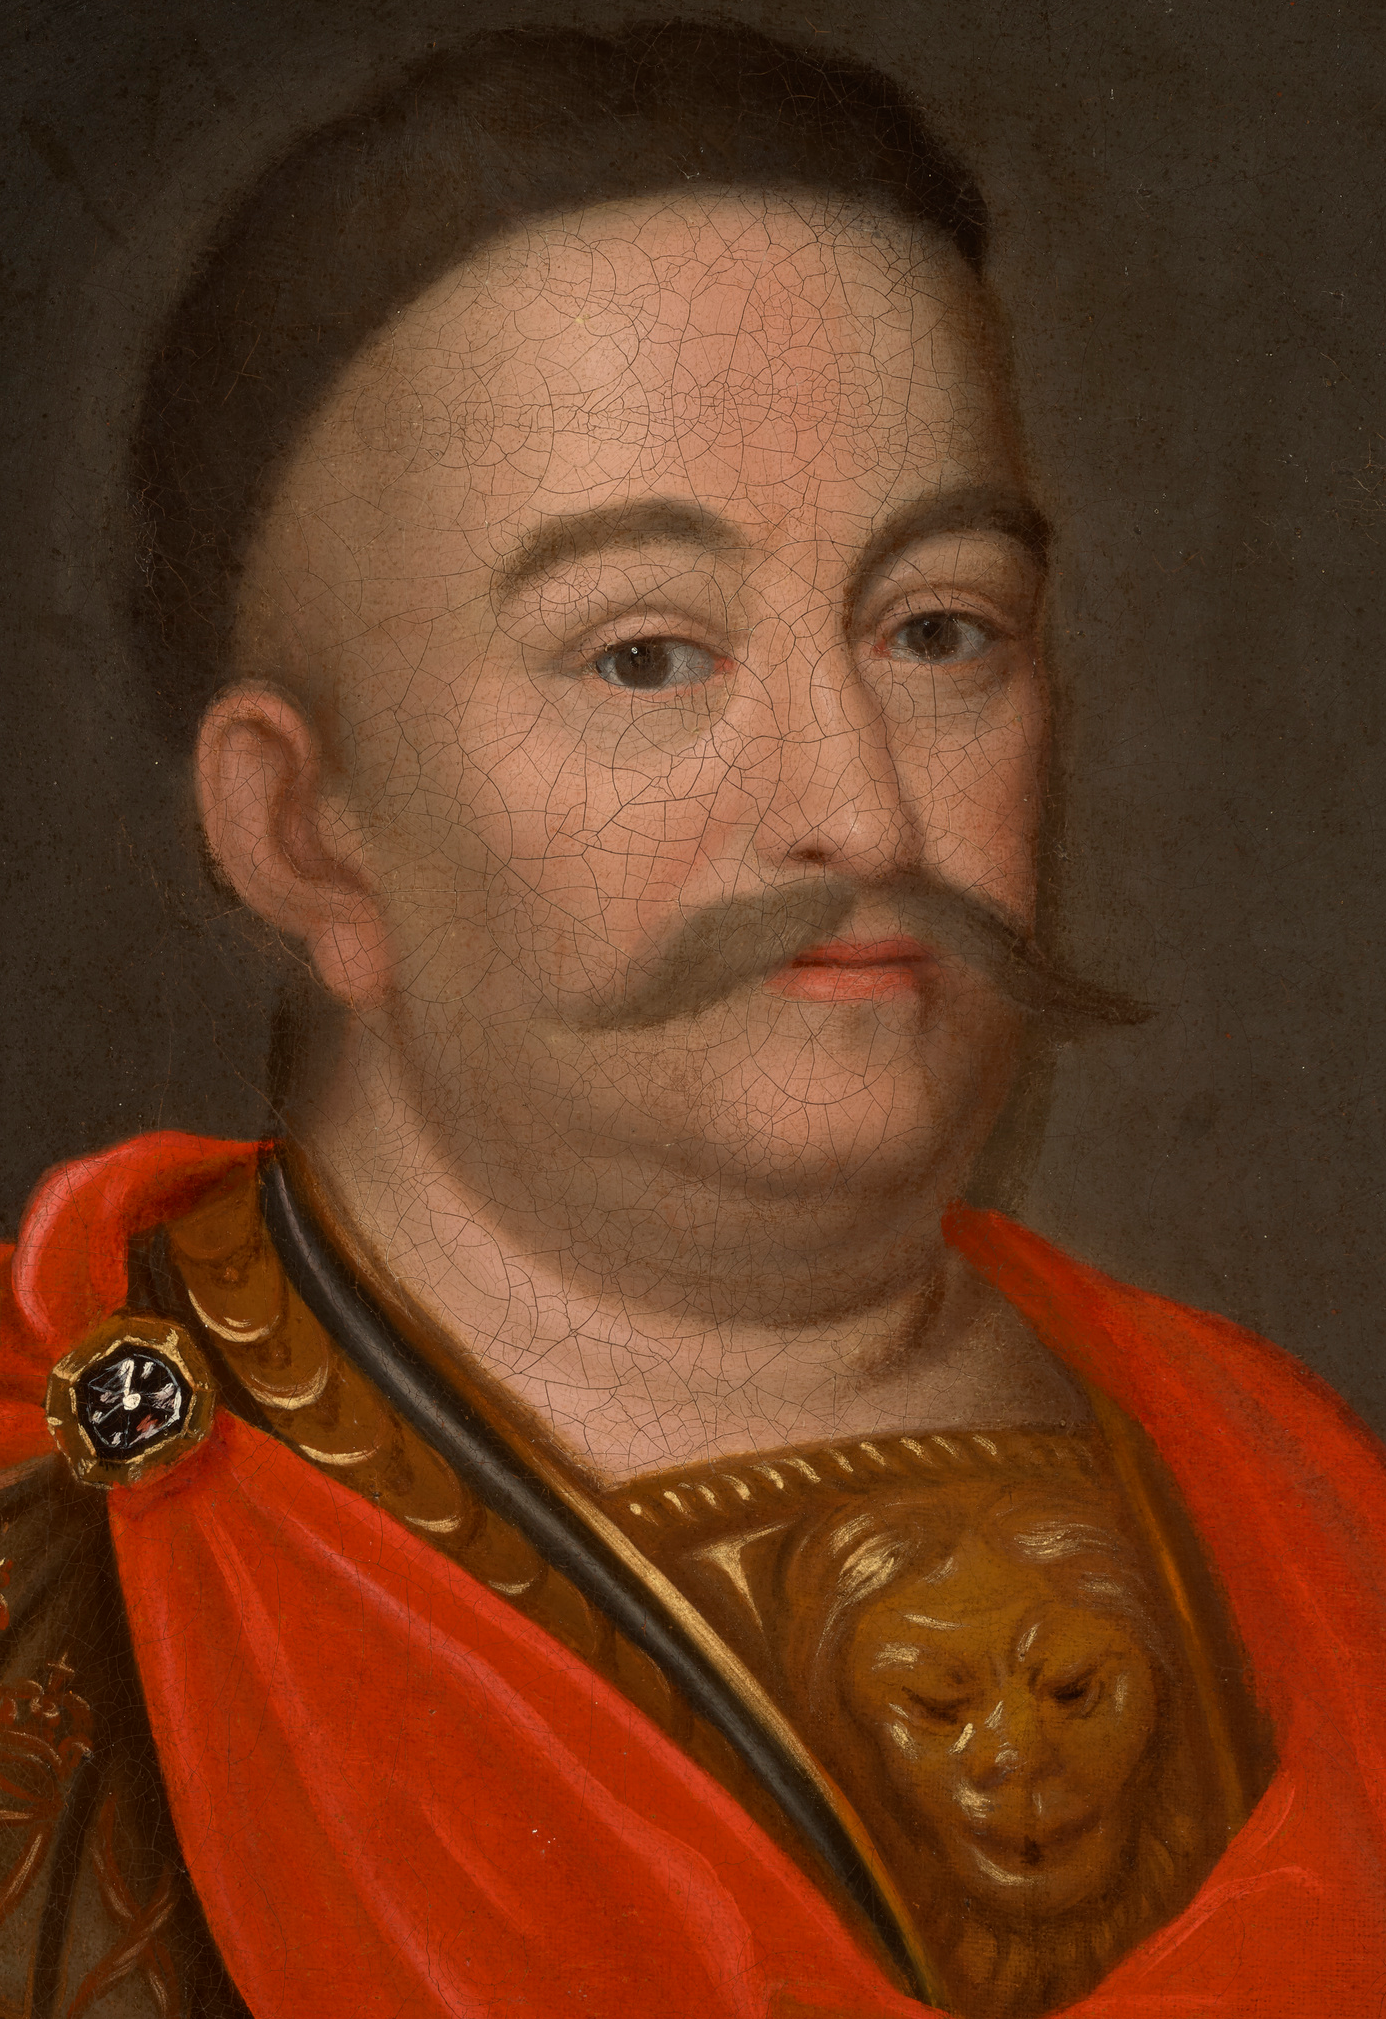
\includegraphics[width=0.5\textwidth]{img/jan_sobieski_w_karacenie.png} 
  \caption{An examined fragment of ``Portrait of John III Sobieski in Karacena Scale Armour''. Source: \cite{wikimediaSobieskiPortrai} }
  \label{fig:sobieski_fragment}
\end{figure}

\subsubsection{Clusterization With SOM}
The first clustering algorithm, SOM, was invoked as presented in \prettyref{lst:som-invocation}.
\newenvironment{longlistingG}{\captionsetup{type=listing, width=0.8\textwidth}}{}
\begin{longlistingG}
    \pythoncode{listings/som_invocation.py}
    \caption{Invocation of SOM algorithm}
    \label{lst:som-invocation}
\end{longlistingG}
\vspace{12pt}

The arguments used to initialize \texttt{SelfOrganizingMap} are:
\begin{description}
    \item[\texttt{input\_size}:] Configured to the number of channels (4094 in this instance).
    \item[\texttt{map\_size}:] Set to (3, 3), indicating a total of $3 \times 3 = 9$ clusters.
    \item[\texttt{learning\_rate}:] The learning rate during the first epoch.
    \item[\texttt{sigma\_neigh}:] The influence on the neighbors of the BMU. Lower values result in larger influence.
    \item[\texttt{sigma\_decay}:] The rate of decay for the learning rate. Lower values result in slower decay.
\end{description}
The performance of the algorithm scales linearly with the number of clusters. 
With a total of 9 clusters, the clusterization of data with shape of (524, 348, 4094) takes approximately 6 minutes. 
Therefore, it may not be feasible method if many more clusters were needed, at least while using basic python implementation and performing clusterization globally.

The result of applying clusterization on raw spectrum can be observed on \prettyref{fig:sobieski_clustered_som_noise}.

\newpage
\begin{figure}[H] 
  \centering     
  \includesvg[width=1\textwidth]{img/sobieski_clustered_som_noise.svg} 
  \caption{Clusterization of unprocessed spectrum of ``Portrait of John III Sobieski in Karacena Scale Armour'' using SOM}
  \label{fig:sobieski_clustered_som_noise}
\end{figure}

As the reader may notice, certain clusters are just artifacts. 
It was sensible to investigate the possibility of these artifacts arising from a poor implementation of the SOM algorithm (although it was not the best first course of action). 
This involved employing a UMAP to HDBSCAN pipeline to validate the clustering results.

\subsubsection{Clusterization With UMAP And HDBSCAN}
Clusterization with UMAP and HDBSCAN was invoked as presented in \prettyref{lst:umap-hdbscan-invocation}.

\newenvironment{longlistingH}{\captionsetup{type=listing, width=0.8\textwidth}}{}
\begin{longlistingH}
    \pythoncode{listings/umap_hdbscan_invocation.py}
    \caption{Invocation of UMAP to HDBSCAN pipeline}
    \label{lst:umap-hdbscan-invocation}
\end{longlistingH}
\vspace{12pt}

The meaning of arguments passed to UMAP is as follows:
\begin{description}
    \item[\texttt{n\_neighbors:}] The number of neighbors used for manifold approximation. As \texttt{n\_neighbors} increases more focus is placed on the global structure of the data. 
    \item[\texttt{min\_dist:}] The minimum distance between points in the dimensional embedding. For clusterization, values around 0 are preferred, because it is desirable to transform data into "tightly packed" clumps.
    \item[\texttt{n\_components:}] The number of dimensions in the low-dimensional representation. Experimentation showed that reducing dimensions to one gave the best results. 
\end{description}

Arguments for HDBSCAN are:
\begin{description}
    \item[\texttt{min\_samples:}] The number of samples in a neighborhood for a point to be considered a core point.
    \item[\texttt{min\_cluster\_size:}] The minimum number of points required to form a cluster. It is probably the most important parameter; smaller values will lead to more clusters.
    \item[\texttt{metric:}] The distance metric used for clustering. Euclidean distance works well, although other popular metrics give good results too.
\end{description}

Dimensionality reduction using UMAP took approximately 7 minutes. 
The cost scales with the parameter \texttt{n\_neighbors}.
Further clusterization with HDBSCAN is much faster (due to the really low dimensionality of input) and allows for fast experiments with different parameters, e.g. to achieve the desired granularity of clusters.

It appears that although clusterization worked, it did not prevented artifacts from appearing - see \prettyref{fig:sobieski_clustered_hdbscan_noise}.
\begin{figure}[H] 
  \centering     
  \includesvg[width=1\textwidth]{img/sobieski_clustered_hdbscan_noise.svg} 
  \caption{Clusterization of unprocessed spectrum of ``Portrait of John III Sobieski in Karacena Scale Armour'' using UMAP and HDBSCAN}
  \label{fig:sobieski_clustered_hdbscan_noise}
\end{figure}

\newpage
\subsubsection{Source of Clusterization Artifacts}
The source of clusterization artifacts remains unknown as of today. 
However, due to the nature of the artifacts, they may be attributed to a poorly implemented pinhole camera.
Two possible implementations of a pinhole camera are demonstrated in \prettyref{fig:pinhole-camera-implementations}.

\begin{figure}[H]
  \centering
  \includegraphics[width=0.8\textwidth]{img/pinhole_camera.png}
  \caption{1-hole pinhole camera (left) and 4-hole pinhole camera (right). Source: \cite{Lach2022}}
  \label{fig:pinhole-camera-implementations}
\end{figure}

The details of the pinhole camera implementation used during measurements are unknown, but the artifacts strongly suggest that a 4-hole pinhole camera was used. 
It seems that differences between pinhole cameras lead to different artifacts showing up during clusterization. 
Fortunately, the clusterization problem turned out to is easily solvable.

\newpage
\subsubsection{Clusterization Results}
By simply removing one hundred points from both ends of the spectrum, the results of clusterization were tremendously improved, as visible in \prettyref{fig:som-clusterization-clean} and \prettyref{fig:hdbscan-clusterization-clean}.

\begin{figure}[H]
  \centering
  \includesvg[width=1\textwidth]{img/sobieski_clustered_som_clean.svg}
  \caption{Clusterization of the cropped spectrum of ``Portrait of John III Sobieski in Karacena Scale Armour'' using SOM.}
  \label{fig:som-clusterization-clean}
\end{figure}

\begin{figure}[H]
  \centering
  \includesvg[width=1\textwidth]{img/sobieski_clustered_hdbscan_clean.svg}
  \caption{Clusterization of the cropped spectrum of ``Portrait of John III Sobieski in Karacena Scale Armour'' using UMAP and HDBSCAN.}
  \label{fig:hdbscan-clusterization-clean}
\end{figure}

\newpage
To better understand the clusters they can be visualized on separate pictures, as shown in \prettyref{fig:som-clusters-clean} and \prettyref{fig:hdbscan-clusters-clean}.
\begin{figure}[!htbp]
  \centering
  \includesvg[width=0.8\textwidth]{img/sobieski_clusters_som_clean.svg}
  \caption{Separate clusters from SOM clusterization}
  \label{fig:som-clusters-clean}
\end{figure}

\begin{figure}[!htbp]
  \centering
  \includesvg[width=0.8\textwidth]{img/sobieski_clusters_hdbscan_clean.svg}
  \caption{Separate clusters from UMAP and HDBSCAN clusterization}
  \label{fig:hdbscan-clusters-clean}
\end{figure}


\newpage
Spectra from each cluster can be accumulated and preprocessed (as was discussed in \prettyref{sec:data-preprocessing})  before being passed to classifier - see \prettyref{fig:som-spectra} and \prettyref{fig:hdbscan-spectra}.

\begin{figure}[!htbp]
  \centering
  \includesvg[width=1\textwidth]{img/sobieski_spectra_som_clean.svg}
  \caption{Processed spectra from SOM clusterization}
  \label{fig:som-spectra}
\end{figure}

\begin{figure}[!htbp]
  \centering
  \includesvg[width=1\textwidth]{img/sobieski_spectra_hdbscan_clean.svg}
  \caption{Processed spectra from UMAP and HDBSCAN clusterization}
  \label{fig:hdbscan-spectra}
\end{figure}
\subsection{Training ViT}
Results visible in next pages were obtained using ViT model trained with the hyperparameters visible on \prettyref{lst:vit-hyperparameters}.

\newenvironment{longlistingI}{\captionsetup{type=listing, width=0.8\textwidth}}{}
\begin{longlistingI}
    \pythoncode{listings/vit_hyperparameters.py}
    \caption{ViT model initialization}
    \label{lst:vit-hyperparameters}
\end{longlistingI}
\vspace{12pt}

For the training phase, 90,000 samples were generated, comprising 10,000 samples for different number of elements ranging from 0 to 9. 
90\% of the samples were utilized in the training step, while the remaining 10\% were allocated for the validation. 
The Adam optimizer was employed with a learning rate of 0.0001, and Binary Cross Entropy loss was used because multi-label classification reduces to multiple binary classification problems.

The model was trained for 10 epochs, with a batch size of 128. 
Loss through epochs can be seen on \prettyref{fig:vit-loss}. 
Training loss was averaged over all mini batches in epoch, which is why it is generally larger than validation loss, which was calculated after the epoch. 

After training, the ROC (Receiver Operating Characteristics) curve over 5000 random samples was calculated to assess the model's performance. 
The ROC curve is a plot of recall (sensitivity) against $1-\text{specificity}$ \cite{rocCurve}.
Recall, also known as the TPR (True Positive Rate) measures the ability of a model to capture all the relevant instances and is defined as \(\frac{\text{TP}}{\text{TP} + \text{FN}}\) (look \prettyref{tab:classification_matrix} for abbreviations).
$1-\text{specificity}$, or FPR (False Positive Rate) is defined as \(1 - \frac{\text{TN}}{\text{TN} + \text{FP}}\) and says what proportion of actual negative instances is correctly identified as negative.
When the threshold for positive classification, e.g., 0.5, is lowered, the number of positive classifications increases, resulting in an increase of both TPR and FPR. 
However, lowering the threshold will lead to an increase in false positives, possibly greater than true positives, causing the \(\frac{\text{TPR}}{\text{FPR}}\) ratio to decrease.

In general, better classifiers should have a greater area under the ROC curve, known as AUC (Area Under the Curve). 
The ROCs and AUCs were calculated using the best weights of the trained model and are visible in \prettyref{fig:roc-auc}.

\begin{table}[htbp!]
  \centering
  \begin{tabular}{|c|c|c|}
    \hline
    & \textbf{Real Positive} & \textbf{Real Negative} \\
    \hline
    \textbf{Predicted Positive} & True Positive (TP) & False Positive (FP) \\
    \hline
    \textbf{Predicted Negative} & False Negative (FN) & True Negative (TN) \\
    \hline
  \end{tabular}
  \caption{Classification matrix}
  \label{tab:classification_matrix}
\end{table}

\begin{figure}[htbp!]
  \centering
  \includesvg[width=0.8\textwidth]{img/vit_loss.svg}
  \caption{Loss in each training epoch}
  \label{fig:vit-loss}
\end{figure}

ROC of a few elements, namely Ca, K, Sn, and Sb, seems to differ significantly from the rest. 
The energies of their spectral lines are as follows: 3.692, 3.314, 3.444, and 3.604 [keV]. 
As one can see, these values are quite close to each other, and the elements do not have any other lines defined in the code that could help differentiate between elements.
In that case model could be improved by using more accurate theoretical element spectra. 

Besides ROC, a few metrics were evaluated for different number of elements in spectra, namely: accuracy, precision, recall and f1 score. 
Precision measures the accuracy of the positive predictions and is evaluated as $\frac{TP}{FP+TP}$ .
f1 score is popular metric that unifies precision and recall under one metric evaluated as a harmonic mean -  $2\times\frac{precision \times recall}{precision + recall}$.
The evaluation was conducted on 1000 random samples within each category and is visible on \prettyref{fig:vit-metrics}.

Based on the precision histogram, it can be concluded that the count of false positives grows rapidly with an increase in elements in the spectrum. It is hard to determine how this issue may be mitigated; perhaps the best course of action is to compare results with another method. 
Additionally, besides attempting to improve the existing model, hyperparameters and training process, it may be worthwhile to try training separate classifiers for each element and assess whether such an approach could yield better results.

\begin{figure}[htbp!]
  \centering
  \includegraphics[width=1\textwidth]{img/roc_auc.png}
  \caption{ROC and AUC of each trained element}
  \label{fig:roc-auc}
\end{figure}

\begin{figure}[htbp!]
  \centering
  \includegraphics[width=0.8\textwidth]{img/metrics.png}
  \caption{Metrics for different number of elements in spectrum}
  \label{fig:vit-metrics}
\end{figure}


\subsection{Classifying Spectra}
\subsubsection{Simple Spectrum Classification}
After training the model was tested on a ``base case'', that is accumulated spectrum of copper PCB as shown in \prettyref{fig:spectra-comparison}.
The output probabilities are visible on \prettyref{fig:copper-pcb-classification}.

\begin{figure}[H]
  \centering
  \includesvg[width=0.7\textwidth]{img/spectra-comparison.svg}
  \caption{Real and artificial spectrum comparison}
  \label{fig:spectra-comparison}
\end{figure}


\begin{figure}[H]
  \centering
  \includesvg[width=0.8\textwidth]{img/classification-results.svg}
  \caption{Classification results}
  \label{fig:copper-pcb-classification}
\end{figure}

In this simple case, the results are satisfactory.

\subsubsection{Classification Of Clustered Spectra}
Now, considering that the model is far from ideal, the results of clustered spectra classification will be shown. 
Spectra were clustered, accumulated and preprocessed as presented in \prettyref{sec:clustered-spectra}.
In the last step they were classified and probability maps for each element were visualized.
Due to probabilistic nature the maps they do not provide any quantitative information! 
Results are visible in \prettyref{fig:clusters-prob-sobieski}, \prettyref{fig:clusters-prob-gasecki} and \prettyref{fig:clusters-prob-matka-boska}.

\begin{figure}[htbp!]
  \centering
  \includesvg[width=1\textwidth]{img/prediction_on_clusters_sobieski.svg}
  \caption{Probability maps of clustered spectra of ``Portrait of John III Sobieski in Karacena Scale Armour''}
  \label{fig:clusters-prob-sobieski}
\end{figure}

\begin{figure}[htbp!]
  \centering
  \includesvg[width=1\textwidth]{img/prediction_on_clusters_gasecki.svg}
  \caption{Probability maps of clustered spectra of ``Portrait of Mieczysław Gąsecki''}
  \label{fig:clusters-prob-gasecki}
\end{figure}

\begin{figure}[htbp!]
  \centering
  \includesvg[width=1\textwidth]{img/prediction_on_clusters_matka_boska.svg}
  \caption{Probability maps of clustered spectra of ``Mother of
God with the Child Eating an Apple''}
  \label{fig:clusters-prob-matka-boska}
\end{figure}

As expected, many false positives appeared in probability maps.
On the other hand results are not \emph{very} tragic. 
As one can see in \prettyref{fig:lach-comparison}, Pb was detected pretty well.
Little worse, but Fe was also registered in places of higher concentration.
Cu was mostly registered incorrectly because the escape photons of the $L_{\alpha}$ spectral line of Pb (7.59 keV) have energy close to the $K_{\alpha}$ line (8.05 keV) of Cu. 
This particular line was not included in the training process, so adding it could potentially improve the results.

\begin{figure}[htbp!]
  \centering
  \includegraphics[width=1\textwidth]{img/comparison-lach.png}
  \caption{Comparison of probability maps with element distribution maps from \cite{Lach2022}}
  \label{fig:lach-comparison}
\end{figure}

\subsubsection{Classification Of Small Regions}
Another option was to classify single spectra or spectra averaged over small regions, e.g. $10\times10$ points. 
Savitzky–Golay filter was used to smooth spectra before further processing.
Also, extrapolation step was omitted during preprocessing to reduce computational cost.
Example spectra are shown in \prettyref{fig:spectra}.

\begin{figure}[H]
    \begin{subfigure}{.5\linewidth}
        \centering
        \includesvg[width=1\textwidth]{img/spectrum_1x1.svg}
        \caption{Single spectrum }
        \label{fig:sub1}
    \end{subfigure}%
    \begin{subfigure}{.5\linewidth}
        \centering
        \includesvg[width=1\textwidth]{img/averaged_spectrum_processing_5x5.svg}
        \caption{Spectrum averaged over $5\times5$ region}
        \label{fig:sub2}
    \end{subfigure}\\[1ex]
    \centering
    \begin{subfigure}{0.5\linewidth}
        \centering
        \includesvg[width=1\textwidth]{img/averaged_spectrum_processing_10x10.svg}
        \caption{Spectrum averaged over $10\times10$ region}
        \label{fig:sub3}
    \end{subfigure}
    \caption{Example spectra}
    \label{fig:spectra}
\end{figure}

Resulting probability maps for different options are shown in \prettyref{fig:10x10-point-sobieski}, \prettyref{fig:5x5-point-sobieski} and \prettyref{fig:single-point-sobieski}.

\begin{figure}[htbp!]
  \centering
  \includesvg[width=1\textwidth]{img/prediction_on_averaged_segments_10x10_sobieski.svg}
  \caption{Probability maps calculated over $10\times10$ segments of ``Portrait of John III Sobieski in Karacena Scale Armour''}
  \label{fig:10x10-point-sobieski}
\end{figure}

\begin{figure}[htbp!]
  \centering
  \includesvg[width=1\textwidth]{img/prediction_on_averaged_segments_5x5_sobieski.svg}
  \caption{Probability maps calculated over $5\times5$ segments of ``Portrait of John III Sobieski in Karacena Scale Armour''}
  \label{fig:5x5-point-sobieski}
\end{figure}

\begin{figure}[htbp!]
  \centering
  \includesvg[width=1\textwidth]{img/prediction_on_single_spectra.svg}
  \caption{Probability maps calculated over single points of ``Portrait of John III Sobieski in Karacena Scale Armour''}
  \label{fig:single-point-sobieski}
\end{figure}
\section{Conclusion}
In conclusion, this engineering thesis has sought to address problem of classifying elements present in XRF spectra. 





\bibliography{bibliography.bib}
\bibliographystyle{plainnat} 
\end{document}
